%% ========================================================================
%%							NNLS
%% ========================================================================


\chapter{Neural Networks (NN)}
\label{cha:NN}

In the last chapter of this thesis, a mathematical concept is discussed that has attracted much attention in the recent past, namely neural networks. The area of artificial intelligence (AI) in which neural networks are embedded has been the subject of an intense media hype in recent years. In 2016, for example, a computer program developed by the British company Google DeepMind succeeded for the first time in defeating Lee Sedol of South Korea, considered to be the strongest Go player in the world \cite{wiki_01}. This victory of a machine against a human being is considered to be a milestone in the field of artificial intelligence \cite{LA_Times}. Further successes were also achieved in the area of real-time games at the beginning of 2019. For the first time DeepMind's program called AlphaStar was able to defeat the world's best players in StarCraft which is considered to be one of the most challenging real-time strategy games \cite{AlphaStar}. Also Gartner, a global research and advisory firm, which publishes the well-known but definitely criticisable hype cycle representations considers AI as one of the most important technologies of recent years. In the hype cyle for emerging technologies from 2017 there are 4 out of the 32 listed technologies that can be attributed to the field of AI, such as Deep Learning or Machine Learning \cite{Gartner2017}. Also in the following years 2018 and 2019 technologies that clearly belong to the AI sector were mentioned in the hype cycle 5 and 6 times respectively \cite{Gartner2018}, \cite{Gartner2019}. This trend towards new methods based on neruonal networks can also be seen in other places, such as Kaggle. With more than one million registered users, Kaggle is one of the world's largest platforms for data science competitions and attracts teams from all over the world with prize money in the millions \cite{Kaggle}. It can be observed that, besides gradient boosting, one of the most important concepts with which to win Kaggle competitions is the concept of neural networks in various forms.   

It is therefore clear to see that on the one hand the technology behind AI has enormous potential to solve problems that have so far been assumed to be solved only by humans. On the other hand, it can be assumed that this trend is not just a short-lived phenomenon, but a continuous process leading to business solutions which are based on AI-systems. Therefore, it is even more important to understand the underlying concepts of these technologies and to discuss their applicability in the insurance industry. Whether in the end a completely automated grouping algorithm based on neural networks is possible at all or can be implemented with the available resources remains open. However, the aim is to provide an overview of the basic concepts and to present case studies with insurance cashflows. Since various terms and buzzwords related to artificial intelligence are often used differently in media reports, it is useful to classify some of the most often used terms in order to show their relationship and provide a general framework which is based on \cite{Allaire2018}. 

\begin{figure}
	\centering
	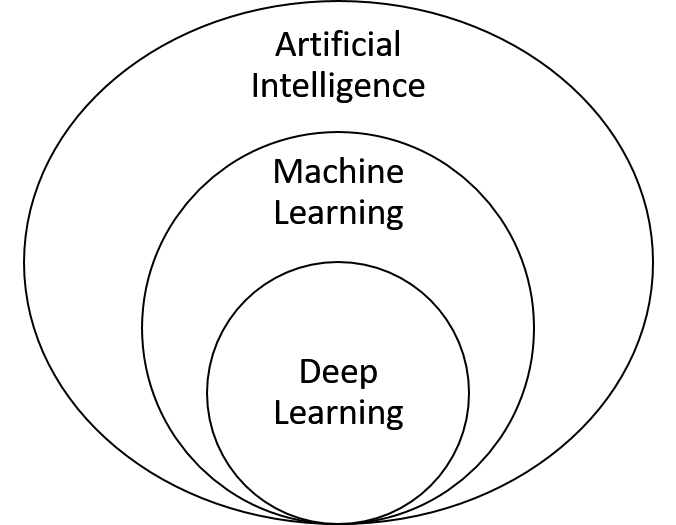
\includegraphics[width=0.5\textwidth]{figures/chapter_NN/framework}
	\caption{Relation of Artificial Intelligence, Machine Learning, and Deep Learning.}
	\label{fig:framework}
\end{figure}

\begin{itemize}
	\item Artificial Intelligence: Artificial Intelligence is a branch of computer science that deals with the programming of intelligent computer systems. Due to a missing definition of the term intelligence the question which types of computer programs are included is not clearly definable. In addition to machine learning and deep learning, there are many other approaches that do not include any kind of learning but are also part of AI. 
	\item Machine Learning: Machine learning arises from this question if it is possible to design a program in such a way that it can learn how to perform a specific task automatically. Given a set of input data and the corresponding results the task is to derive rules. These rules are therefore the output of the machine learning algorithm and can then be used to derive the results for new input data. What all these methods have in common is the fact that they actually try to identify statistical patterns in the data. Thus the aims to find a meaningful representation of the given data by projections, translations or nonlinear transformations and to apply it to new data. 	 
	\item Deep Learning: 
\end{itemize}




